\documentclass{article}

\usepackage{listings}
\usepackage{amsmath}
\usepackage{graphicx}
\usepackage{hyperref}
\usepackage{booktabs}
\usepackage{verbatim}
\usepackage{url}

\begin{document}

\title{Parallel Histogram Calculation in CUDA}
\author{Geoffrey Ulman\\
        CS706}
\date{November 2012}
\maketitle

\section{Abstract}\label{abstract}

Glimpse (\url{http://metsci.github.com/glimpse/}) is a Java library for building 2D data visualization applications which utilize GPU hardware to allow rapid exploration of large data sets\footnote{I have developed Glimpse as part of my professional work over the past year. The development of the graphics library itself is not part of the scope of this project, only the development, profiling, and debugging of the CUDA histogram calculation kernel and the use of Glimpse to visualize the results. Glimpse is released under the open source BSD license.}. For example, Glimpse uses GPU shaders to dynamically color large heat map plots like Figure \ref{histogram1}. However, more complicated data analysis and visualization is better suited for NVIDIA's Compute Unified Device Architecture (CUDA) which exposes GPU hardware for general purpose computation\cite{cuda-zone}.

This project uses CUDA to calculate histograms for subsections of a large heat map in real time and displays the results using Glimpse visualization tools. NVIDIA's Visual Profiler\cite{nvidia-visual-profiler} is used to guide performance optimizations and three versions of the CUDA code are discussed. Profiling and optimizing CUDA applications is difficult because computations are run on hundreds of cores simultaneously. Determining and fixing performance bottlenecks is complicated by multiple interdependent concerns including: fitting kernel register and shared memory usage into available hardware, significant differences in efficient memory access patterns for different memory spaces (global, constant, and shared memory), managing synchronization of hundreds of GPU threads, and generally tight coupling of low-level hardware considerations to algorithm design.

The input data to the histogram calculation is a matrix of floating point data values. The output is an array of integers containing the number of matrix values which fall within a set of discrete bins. The matrix data is stored in video memory as a two dimensional OpenGL texture. This allows CUDA to take advantage of specialized caching hardware on the graphics card to speed data access. Figure \ref{histogram1} shows the final Java visualization application and Section \ref{visualization} provides a link to a video of the histogram dynamically adjusting in response to user input.

\begin{figure}
\centering
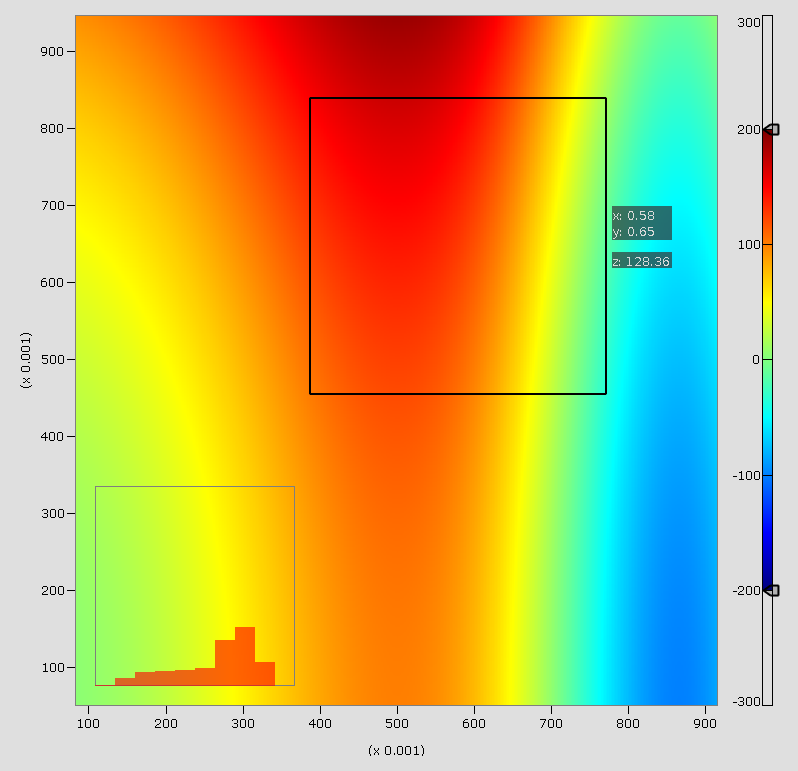
\includegraphics[width=1.0\textwidth]{screenshots/glimpse/GlimpseHistogramPlot.png}
\caption{Glimpse Histogram Visualization}
\label{histogram1}
\end{figure}

\section{Single Threaded Baseline}\label{baseline}

A simple \emph{C} program which calculates histogram bins on a single thread on the CPU was used to establish a performance baseline. A snippet of the histogram calculation is provided in Listing \ref{singlehist1} and the full text of the program is available on GitHub at \url{https://github.com/ulmangt/cs706project/blob/master/src/main/c/histogram_test_nocuda.c}.

The total execution time on an Intel Core i7-980X 3.33 GHz processor was approximately 20 milliseconds for a 1000 row by 1000 column matrix. GPU profiling was performed with a GeForce GTX 480 with 1535 MB of global memory, 15 multiprocessors (each with 32 cores for a total of 480 cores), and a 1.40 GHz clock speed\cite{geforce480}.

\lstset{language=C,basicstyle=\footnotesize}
\begin{minipage}{\textwidth}
\begin{lstlisting}[caption={Single Threaded Histogram Calculation},label={singlehist1}]
  for ( i = 0 ; i < width * height ; i++ )
  {
    // retrieve a data value
    float data = imageData[i];

    // calculate histogram bin index for the data value
    float fbinIndex = floor( ( data - minZ ) / stepZ );
    int binIndex = (int) clamp( fbinIndex, 0, numBins-1 );

    // increment the histogram bin
    bins[binIndex] += 1;
  }
\end{lstlisting}
\end{minipage}

\section{Approach One}\label{approach1}

CUDA \emph{kernels} define the behavior of a single logical GPU thread. Threads are grouped into logical \emph{blocks} and threads in the same \emph{block} can share memory and synchronize with one another. They are physically executed on GPU multiprocessors which execute the same instruction on a \emph{warp} of 32 threads simultaneously. Multiprocessor cores have no branch prediction or speculative execution hardware. Instead, they rely on swapping out warps which are blocked on memory access or slow operations to keep the multiprocessor busy. 

Because of this Single Instruction Multiple Thread (SIMT) data parallel programming model, often the first question which must be asked when designing a CUDA algorithm is how GPU threads will map to data. For the histogram calculation problem, the simplest approach is to simply assign one thread to each matrix/texture element. Each thread determines the appropriate bin for its data value and increment the bin by one.

\lstset{language=C,basicstyle=\footnotesize}
\begin{minipage}{\textwidth}
\begin{lstlisting}[caption={calculateHistogram1: Global Memory atomicAdd},label={kernel1}]
extern "C" __global__ void calculateHistogram1( int *bins, int nbins,
                                                float minX, float stepX,
                                                float minY, float stepY,
                                                float minZ, float maxZ )
{
  // use block and thread ids to get texture coordinates for this thread
  int i = blockIdx.x * blockDim.x + threadIdx.x;
  int j = blockIdx.y * blockDim.y + threadIdx.y;

  // convert block/thread ids into texture coordinates
  float x = minX + stepX * i;
  float y = minY + stepY * j;

  // don't over count if texture coordinates are out of bounds
  if ( x < 1.0 && y < 1.0 )
  {
    // perform texture lookup
    float result = tex2D(texture_float_2D, x, y);

    // calculate bin index
    float stepZ = ( maxZ - minZ ) / nbins;
    float fbinIndex = floor( ( result - minZ ) / stepZ );
    int binIndex = (int) clamp( fbinIndex, 0, nbins-1 );

    // atomically add one to the bin corresponding to the data value
    atomicAdd( bins+binIndex, 1 );
  }
}
\end{lstlisting}
\end{minipage}

Listing \ref{kernel1} contains the kernel which implements this approach. The full code is also available on GitHub at \url{https://github.com/ulmangt/cs706project/blob/master/src/main/c/histogram_test.cu}. The key line in the CUDA kernel in Listing \ref{kernel1} is the \emph{atomicAdd} function call. Each thread, after calculating the bin index for the matrix value it has been assigned, must increment the histogram count array \emph{bins} by 1. However, just like incrementing a shared variable in a multi-threaded \emph{c} program, care must be taken that interleaving of machine instructions does not result in lost increments.

Fortunately, CUDA makes ensuring mutually exclusive access to shared variable easy using the \emph{atomicAdd} operation\cite{arithmetic-functions}. Unfortunately, simplistic use of \emph{atomicAdd} on a variable in \emph{global memory} causes significant performance problems for the \emph{calculateHistogram1} kernel. Figure \ref{kernel1nvvp1} displays an overview screenshot of NVIDIA Visual Profiler (NVVP) results and Figure \ref{kernel1nvvp2} highlights high-level warnings provided by the profiler.

\begin{figure}
\centering
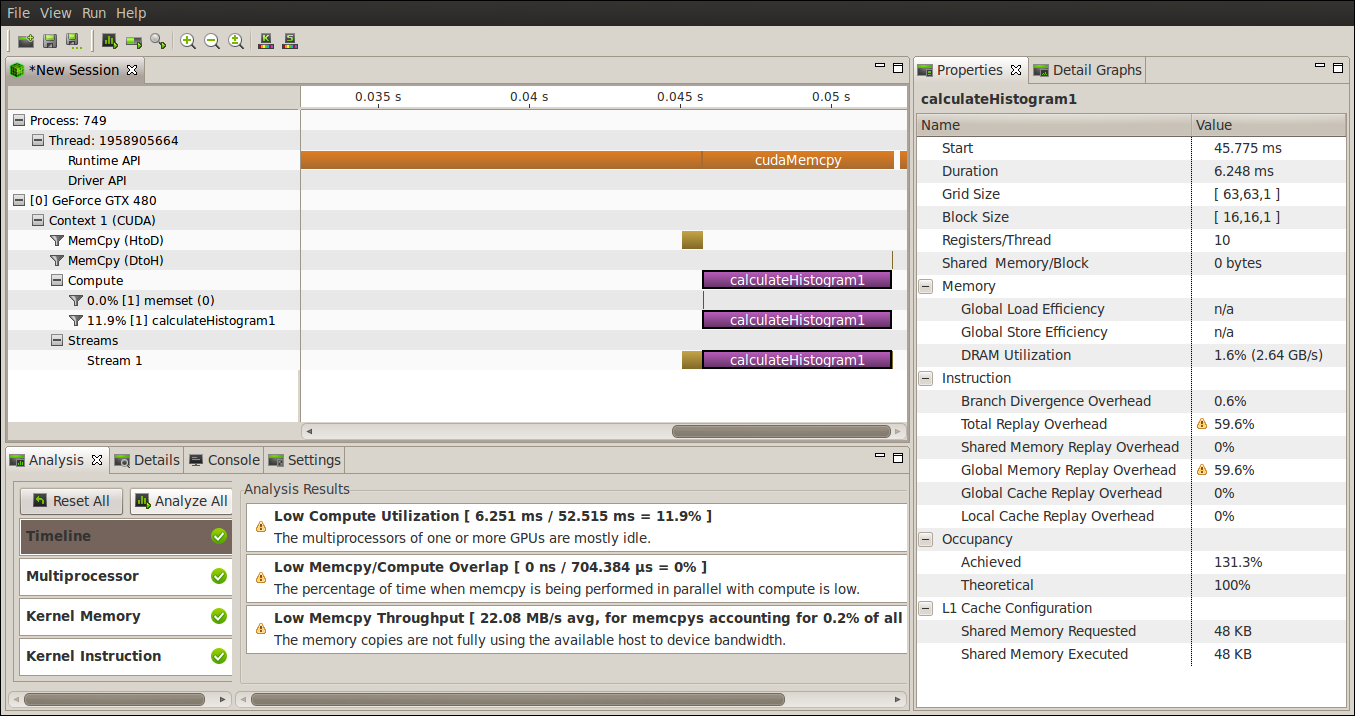
\includegraphics[width=1.0\textwidth]{screenshots/nvvp/calculateHistogram1_screen1.png}
\caption{NVVP calculateHistogram1() Kernel Overview }
\label{kernel1nvvp1}
\end{figure}

\begin{figure}
\centering
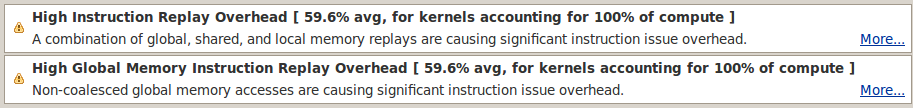
\includegraphics[width=1.0\textwidth]{screenshots/nvvp/calculateHistogram1_screen2.png}
\caption{NVVP calculateHistogram1() Kernel Instruction Analysis}
\label{kernel1nvvp2}
\end{figure}

\begin{figure}
\centering
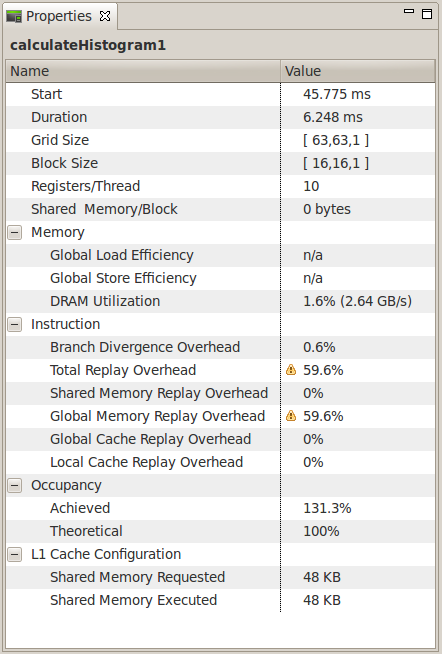
\includegraphics[width=0.65\textwidth]{screenshots/nvvp/calculateHistogram1_screen3.png}
\caption{NVVP calculateHistogram1() Kernel Details}
\label{kernel1nvvp3}
\end{figure}

Instruction replays occur when contention for access to a shared variable by an atomic operation like \emph{atomicAdd} forces the GPU to execute a single operation multiple times. The Visual Profiler indicates that for the approach in Listing \ref{kernel1}, 59.6\% of kernel execution time was taken up by instruction replay and the average kernel execution time was 6248$\mu$s for a 1000 by 1000 pixel element matrix.

\section{Approach Two}\label{approach2}

In addition to the instruction replays due to concurrent access of identical memory locations, the memory being accessed by \emph{atomicAdd} in \emph{calculateHistogram1} was global memory. Global GPU memory is large: on the GeForce GTX 480 there is 1.5 GB of global memory but only 48 KB of shared memory per block\cite{geforce480}. Global memory also has the advantage of being accessible by all thread blocks in a CUDA kernel, whereas shared memory is local to the threads within a single block. However, loading a value from global memory takes about 400 clock cycles, compared to only 4 clock cycles for shared memory\cite{shared-memory}.

Listing \ref{kernel2} contains a modified histogram calculation kernel which attempts to speed up the compuation by utilizing shared memory. The calculation is similar, except that each block produces its own partial histogram, which must then be combined (this step is fast, and is performed on the CPU for simplicity). However, once a block's partial histogram is built in shared memory, it must still be copied to global memory before it can be moved to the CPU. This requires use of the \emph{\_\_syncthreads()} barrier function, which ensures that all threads \emph{in a block} reach the barrier before proceeding. Without this, we might start to copy histogram bins from shared memory to global memory before all threads had finished updating the shared memory histogram bins.

The NVVP results in Figure \ref{kernel2nvvp1} indicate that the overall kernel execution time for this approach decreased to 899$\mu$s. The instruction replay overhead which caused performance problems for Listing \ref{kernel1} is gone. The \emph{atomicAdd} operation is still used, but it is now writing into memory for a sub-histogram shared by 256 other threads (the block size used), instead of a single array of global memory shared by the over 1 million threads among all 3969 blocks. This results in far less memory contention. However, the two branches where only a few threads from each block zero out the shared memory bins and copy the shared memory bins back to global memory mean that most threads simply sit idle during those steps. This is reported by the NVVP in Figure \ref{kernel2nvvp3} as high divergent branch overhead.

\lstset{language=C,basicstyle=\footnotesize}
\begin{minipage}{\textwidth}
\begin{lstlisting}[caption={calculateHistogram2: Shared Memory atomicAdd},label={kernel2}]
extern "C" __global__ void calculateHistogram2(
                                        int* bins,
                                        float minX, float stepX,
                                        float minY, float stepY,
                                        float minZ, float maxZ )
{
  __shared__ int localBins[numBins];

  // unique index for each thread within its block
  int tid = threadIdx.x + threadIdx.y * blockDim.y;

  // unique index for each block
  int bid = blockIdx.x + blockIdx.y * gridDim.y;

  // i and j are indices into the whole texture for this thread
  int i = blockIdx.x * blockDim.x + threadIdx.x;
  int j = blockIdx.y * blockDim.y + threadIdx.y;

  // convert block/thread ids into texture coordinates
  float x = minX + stepX * i;
  float y = minY + stepY * j;

  // clear the shared memory bins (only the first numBins threads)
  if ( tid < numBins )
  {
    localBins[tid] = 0;
  }

  // wait for all shared variable bins for this block to be zeroed
  __syncthreads();

  // don't over count if texture coordinates are out of bounds
  if ( x < 1.0 && y < 1.0 )
  {
    // perform texture lookup
    float result = tex2D(texture_float_2D, x, y);

    // calculate bin index
    float stepZ = ( maxZ - minZ ) / numBins;
    float fbinIndex = floor( ( result - minZ ) / stepZ );
    int binIndex = (int) clamp( fbinIndex, 0, numBins-1 );

    // atomically add one to the bin corresponding to the data value
    atomicAdd( localBins+binIndex, 1 );
  }


  // wait for all threads in this block to finish incrementing their bin
  __syncthreads();

  // the first numBins threads each write out one shared bin to global memory
  if ( tid < numBins )
  {
    bins[bid*numBins+tid] = localBins[tid];
  }
}
\end{lstlisting}
\end{minipage}

\begin{figure}
\centering
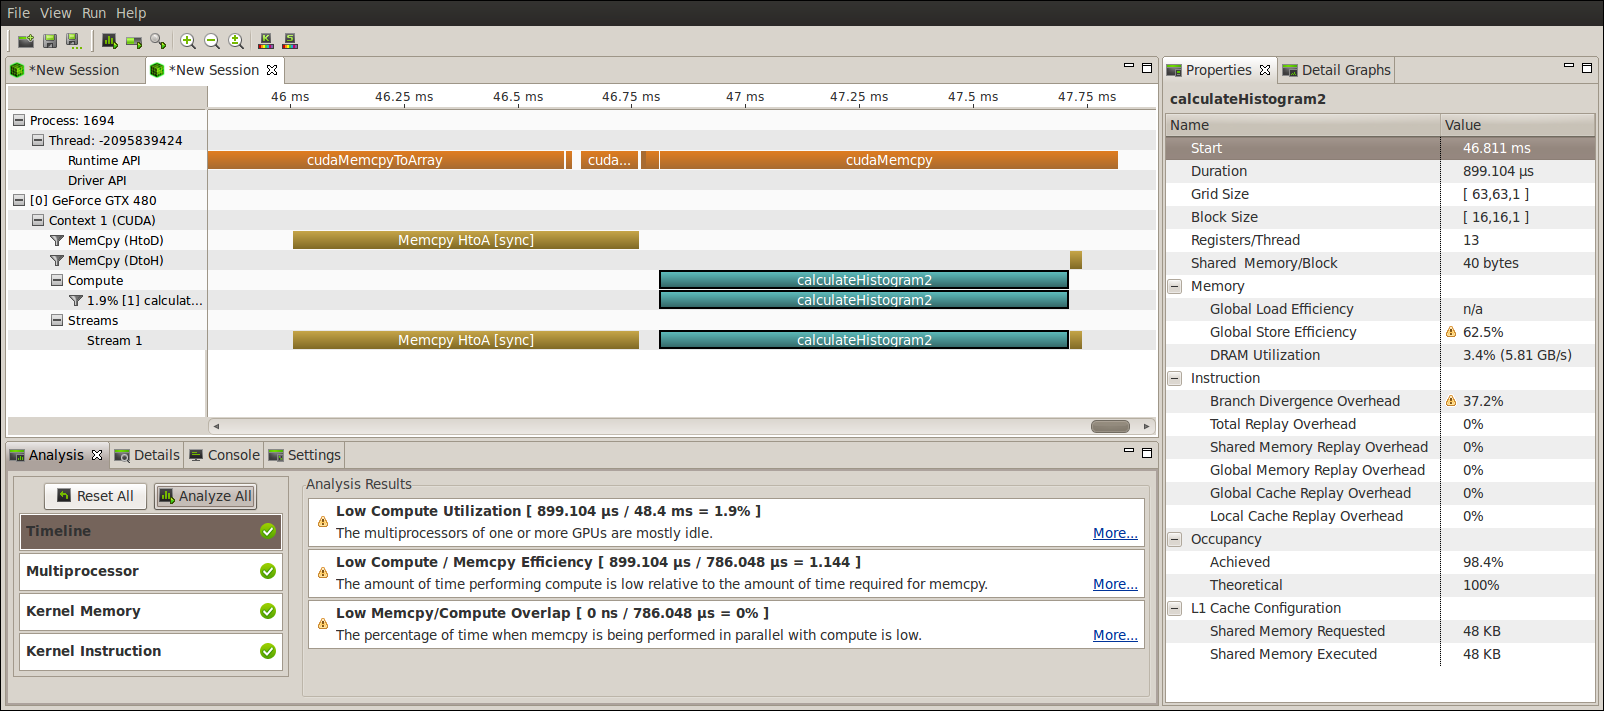
\includegraphics[width=1.0\textwidth]{screenshots/nvvp/calculateHistogram2_screen1.png}
\caption{NVVP calculateHistogram2() Kernel Overview}
\label{kernel2nvvp1}
\end{figure}

\begin{figure}
\centering
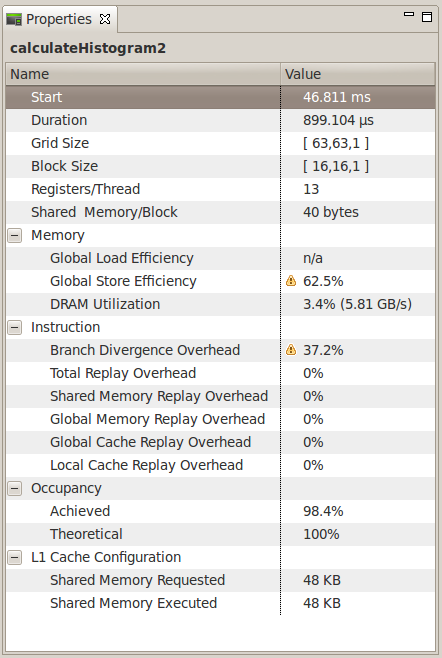
\includegraphics[width=0.65\textwidth]{screenshots/nvvp/calculateHistogram2_screen3.png}
\caption{NVVP calculateHistogram2() Kernel Details}
\label{kernel2nvvp3}
\end{figure}

\section{Approach Three}\label{approach3}

The third approach considered, Listing \ref{kernel3}, eliminates the need for \emph{atomicAdd} entirely by allocating shared memory space for each thread to build its own sub-histogram. Instead of each thread looking up a single texture value, each thread builds a histogram for a small (16 by 16) section of the overall texture. The threads within each block then perform a reduction to combine their per-thread histograms into a single per-block histogram\cite{tree-reduction}. Like Listing \ref{kernel2}, the CPU performs the final step to combine the per-block histograms into a single overall histogram.

\lstset{language=C,basicstyle=\footnotesize}
\begin{lstlisting}[caption={calculateHistogram3: Per-Thread Sub-Histograms},label={kernel3}]
extern "C" __global__ void calculateHistogram3(
                                  int* bins,
                                  float minX, float stepX,
                                  float minY, float stepY,
                                  float minZ, float maxZ )
{
  // allocate enough shared memory for each thread to
  // have its own set of histogram bins
  __shared__ int localBins[numBins*dimBlockx*dimBlocky];

  // unique index for each thread within its block
  int tid = threadIdx.x + threadIdx.y * blockDim.x;

  // unique index for each block
  int bid = blockIdx.x + blockIdx.y * gridDim.x;

  // i and j are indices into the whole texture for this thread
  int i = ( threadIdx.x + blockIdx.x * blockDim.y ) * dimThreadx;
  int j = ( threadIdx.y + blockIdx.y * blockDim.x ) * dimThready;

  int blockSize = dimBlockx*dimBlocky;

  // clear the shared memory bins (only the first numBins threads)
  #pragma unroll
  for ( int k = 0 ; k < numBins ; k++ ) 
  {
    localBins[blockSize*k + tid] = 0;
  }

  #pragma unroll
  for ( int di = 0 ; di < dimThreadx ; di++ )
  {
  #pragma unroll
    for ( int dj = 0 ; dj < dimThready ; dj++ )
    {
      // don't over count if texture coordinates are out of bounds
      if ( di + i < width && dj + j < height )
      {
        // perform texture lookup
        // convert block/thread ids into texture coordinates
        float x = minX + stepX * (i+di);
        float y = minY + stepY * (j+dj);
        float result = tex2D(texture_float_2D, x, y);

        // calculate bin index
        float stepZ = ( maxZ - minZ ) / numBins;
        float fbinIndex = floor( ( result - minZ ) / stepZ );
        int binIndex = (int) clamp( fbinIndex, 0, numBins-1 );

        // no need for atomic operations because each thread
        // is now building its own sub-histogram
        localBins[blockSize*binIndex + tid] += 1;
      }
    }
  }

  // wait for all threads in this block to finish
  // building their sub-histogram
  __syncthreads();

  // perform a tree reduction to combine the
  // sub-histograms on each thread into a single block-histogram
  for ( unsigned int offset = blockSize >> 1; offset > 0; offset = offset >> 1 )
  {
    if ( tid < offset )
    {
      for ( int k = 0 ; k < numBins ; k++ )
      {
        localBins[blockSize*k+tid] += localBins[blockSize*k+tid+offset];
      }
    }

    // synchronize after each tree reduction step
    __syncthreads();
  }

  // at this point, the bin counts for the entire block are in
  // the first numBins entries of localBins
  // now write those bins to global memory
  if ( tid < numBins )
  {
    bins[bid*numBins+tid] = localBins[tid*blockSize];
  }
}
\end{lstlisting}

\begin{figure}
\centering
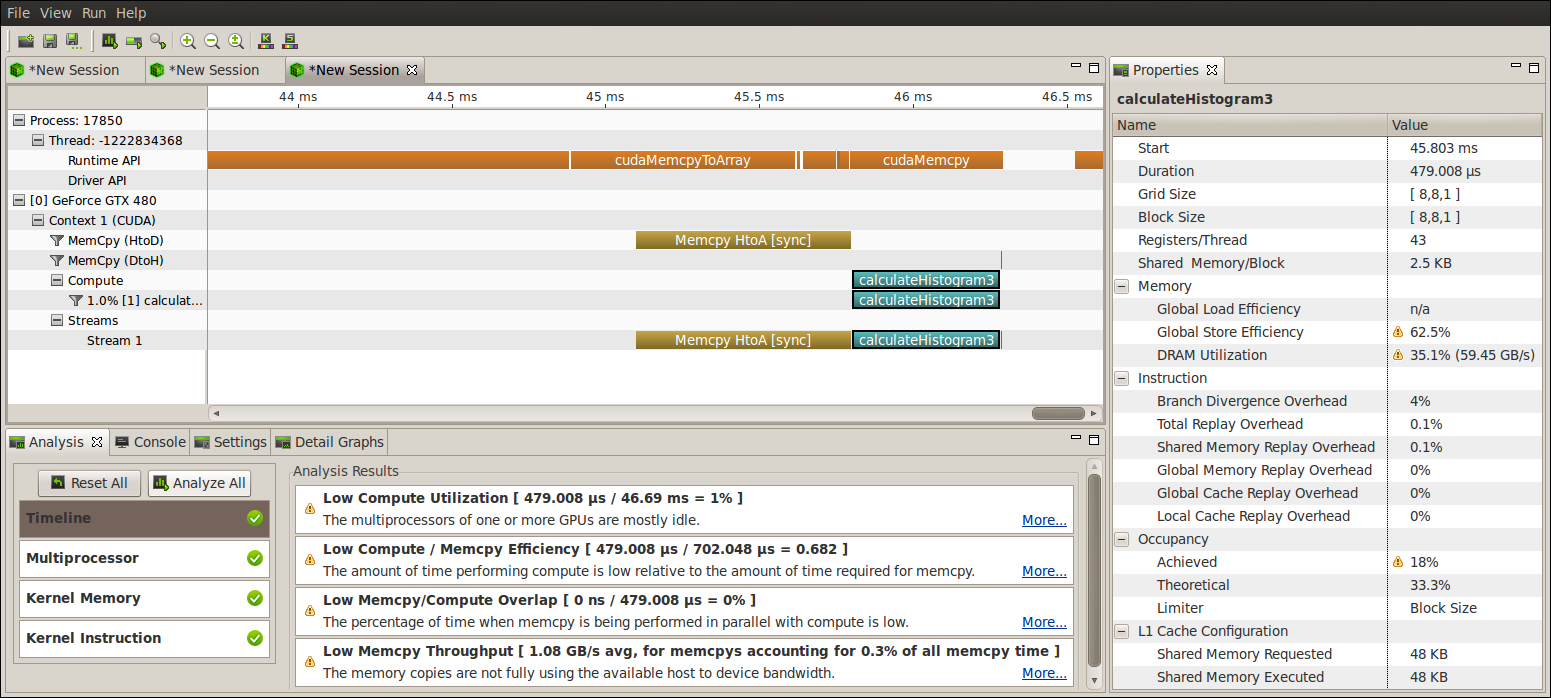
\includegraphics[width=1.0\textwidth]{screenshots/nvvp/calculateHistogram3_screen3.png}
\caption{NVVP calculateHistogram3() Kernel Overview}
\label{kernel3nvvp3}
\end{figure}

\begin{figure}
\centering
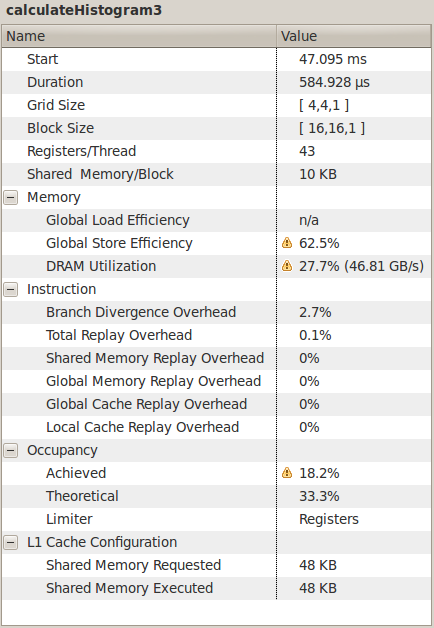
\includegraphics[width=0.65\textwidth]{screenshots/nvvp/calculateHistogram3_screen4.png}
\caption{NVVP calculateHistogram3() Kernel Details}
\label{kernel3nvvp4}
\end{figure}

The NVVP results in Figure \ref{kernel3nvvp3} and Figure \ref{kernel3nvvp4} indicate that this is the fastest approach, taking 584$\mu$s for a 1000 by 1000 pixel element matrix. The main bottlenecks appear to be poor global memory access patterns and low utilization of available multiprocessors (reported as 18.2\% achieved occupancy in the kernel details in Figure \ref{kernel3nvvp4}). Occupancy is defined as the total number of active warps divided by the maximum active warps (which is determined by the number of GPU multiprocessors). Both shared memory and thread registers are limited resources which must be shared among all warps in a block. If individual threads use too many registers or too much shared memory, then processors will sit idle\cite{occupancy}.

In the case of Listing \ref{kernel3}, NVVP reports in Figure \ref{kernel3nvvp4} that register usage is the limiting factor. Unintuitively, in such cases it can often be faster to recalculate a value every time it is needed rather than calculate the value once and store it in a register. A number of adjustments to Listing \ref{kernel3} along those lines were tried, but none had a significant impact on occupancy or overall runtime. Register usage is also affected by compiler loop unrolling, which can be controlled by \emph{\#pragma unroll} directives in the source. However, these also had no impact on occupancy or runtime.

Despite the occupancy issues, \emph{calculateHistogram3} performed significantly better than both other kernels for matrices above 600 pixels per side. Figure \ref{comparison1} provides a runtime comparison for all three kernels (and the single threaded baseline) over a variety of matrix sizes.

\begin{figure}
\centering
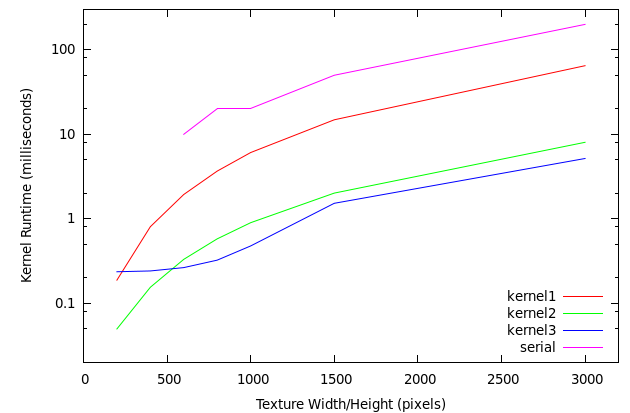
\includegraphics[width=1.0\textwidth]{screenshots/performance.png}
\caption{Kernel Performance Comparison}
\label{comparison1}
\end{figure}

\section{Java Visualization}\label{visualization}

After profiling the CUDA histogram calculation kernel using NVCC, a graphical application written in Java was written to produce an interactive visualization of the histogram calculations (the main motivation for performing the histogram calculations quickly in CUDA was to provide interactive feedback to users). The CUDA kernel is called from Java using JCUDA\cite{jcuda}.

Figure \ref{histogram1} shows the final application. The colors on the heat map plot correspond to data values according to the color scale on the right. The black box indicates the region of the heat map which the user has selected with their mouse. The picture-in-picture histogram plot in the lower left show a histogram of the data values contained within the selected region.

Because compiling and running the project is difficult due to the need to install the CUDA development kit and JCUDA library, a video of the application running is available on Vimeo at \url{https://vimeo.com/54574489} or in the downloads section of the project on GitHub at \url{https://github.com/ulmangt/cs706project/downloads}.

\section{Appendix}\label{appendix}

Full source code for the Java, C, and CUDA portions of this project are available online on GitHub at \url{https://github.com/ulmangt/cs706project}.

\bibliographystyle{plain}
\bibliography{report}

\end{document}
